\section{Adaptive Sampling}
\begin{frame}{Part B}
\Large \center{\color{blue}{Adaptive Sampling Algorithms}}
\end{frame}

\begin{frame}{Idea behind SGD}
According to the SGD theorem, we can reduce the convergence rate by solving the following optimization problem:
\[
    \min \E\big[\|\gv_{i_t}^t\|^2\big].
\]
By the Cauchy-Schwarz inequality and the fact that $\sum_{i=1}^n p_i = 1$,
\[ 
    \E\big[\|\gv_{i_t}^t\|^2\big] = \sum_{i=1}^n \frac{\|\chiv_i\|^2}{n^2p_i} = (\sum_{i=1}^n \frac{\|\chiv_i\|^2}{n^2p_i}) (\sum_{i=1}^n p_i) \ge (\sum_{i=1}^n \frac{\|\chiv_i\|}{n})^2.
\]
The above inequality holds when 
\begin{equation*}\label{eq:p_optimal}
    p_i = \frac{\|\chiv_i\|}{\sum_{j=1}^n \|\chiv_i\|}.
\end{equation*}

\end{frame}

\begin{frame}{AdaSGD}
\begin{figure}[H]
        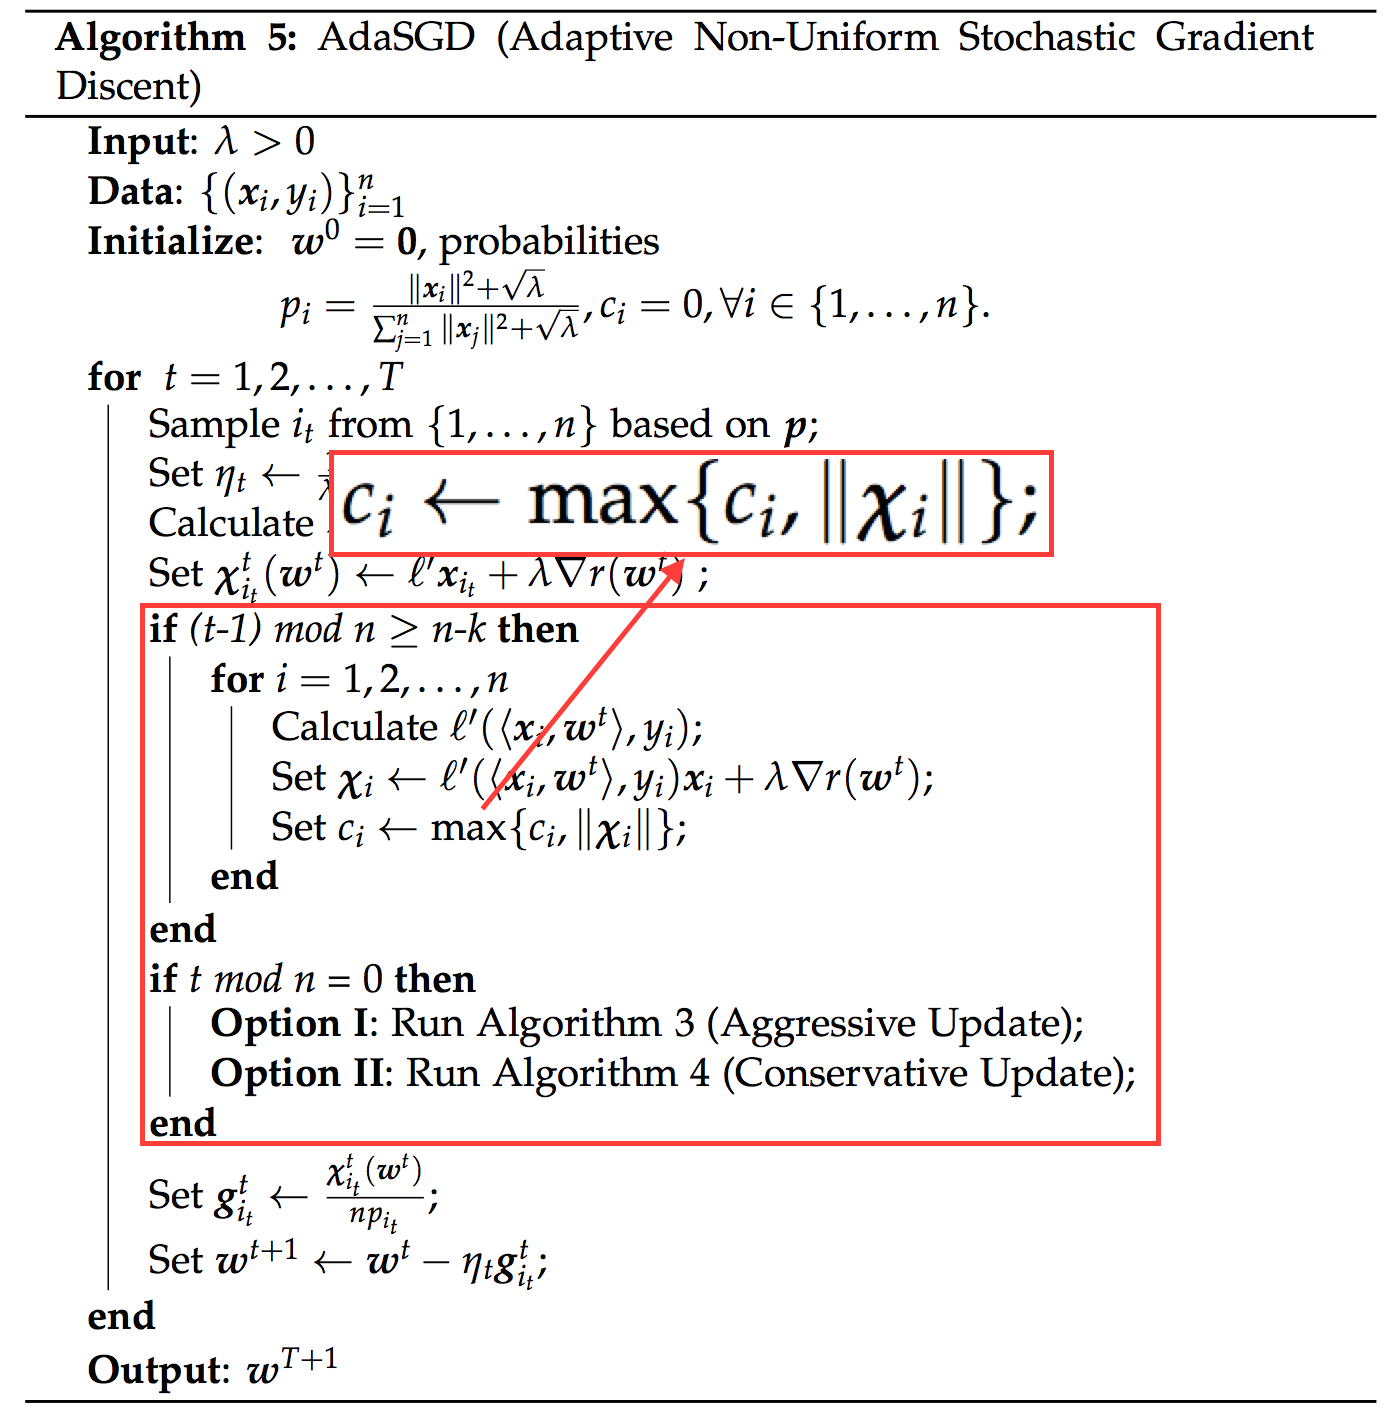
\includegraphics[height=0.8\textheight]{images/AdaSGD.png} 
    \label{fig:AdaSGD}
\end{figure}
\end{frame}

\begin{frame}{Two Updates}
\begin{algorithm}[H]
    \label{alg:AggUpdate}
    \caption{Aggressive Probability Update}
    \SetKwFor{Forloop}{for}{}{end}
    \SetAlgoLined
    \Forloop{$j = 1, \dots, n$} {
	Set $p_j \leftarrow \frac{c_j}{\sum_{k=1}^n c_k}$;
    }
    \end{algorithm}
\begin{algorithm}[H]    
    \label{alg:ConUpdate}
    \caption{Conservative Probability Update}
    \SetKwFor{Forloop}{for}{}{end}
    \SetAlgoLined
    Set $s \leftarrow \sum_{j=1,\dots, n, \1_i=\texttt{0}} c_j$; \\
    Set $c \leftarrow |S|$ where $S \leftarrow \{j | \1_i=\texttt{1}\}$; \\
    \Forloop {$j = 1, \dots, n$} {
	    $p_j>0$ $?$ {$p_j \leftarrow \frac{c_j}{s+c}$} $\colon$ {$p_j \leftarrow \frac{1}{s+c}$; } 
    } 
\end{algorithm} 
\Tiny $\1_i$ is a indicator function which returns $1$ if point $i$ is correctly classified during all the $k$ iterations, otherwise returns $0$.
\end{frame}

\begin{frame}{AdaSVRG}
We add a $\tilde{\wv}$ (which denotes the $\wv$ of last epoch) for a new update equation. Therefore, we get

\begin{equation*}\label{eq:vr_w_update}
    \wv^{t+1} := \wv^{t}-\eta_t [\gv_{i_t}^t(\wv^{t}) - \gv_{i_t}^t(\tilde{\wv}) - \nabla f(\tilde{\wv})]
\end{equation*}

The expectation of the update function is still the same as before, because
\[
    \E[\gv(\wv) - \gv(\tilde{\wv}) + \nabla f(\tilde{\wv})] = \E[\gv(\wv)] - \E[\gv(\tilde{\wv})] + \nabla f(\tilde{\wv}) = \nabla f(\wv).
\]
\end{frame}

\begin{frame}{Idea behind SDCA}
\begin{definition}{Define the gap of point $i$ as} 
\[
\sigma_i^t =  \ell(\xv_i^\intercal\wv^{t})+\ell^*(-\alpha_i^{t})+\alpha_i^{t}\xv_i^\intercal\wv^{t} 
\]
where $\wv^t$ here is assumed to be the corresponding primal vector for the current $\alphav^t$, that is $\wv^t(\alphav^t) := \frac{1}{\lambda n}\sum_{i=1}^n \alpha_i \xv_i^t$.
\end{definition}

The \textbf{duality gap} between the primal objective and dual objective at the $t$-th iteration is defined as
\[
    f(\wv^{t})-D(\alphav^{t}) = \frac{1}{n} \sum_{i=1}^n \sigma_i^t.
\]
\end{frame}

\begin{frame}{AdaSDCA}
\begin{figure}[H]
        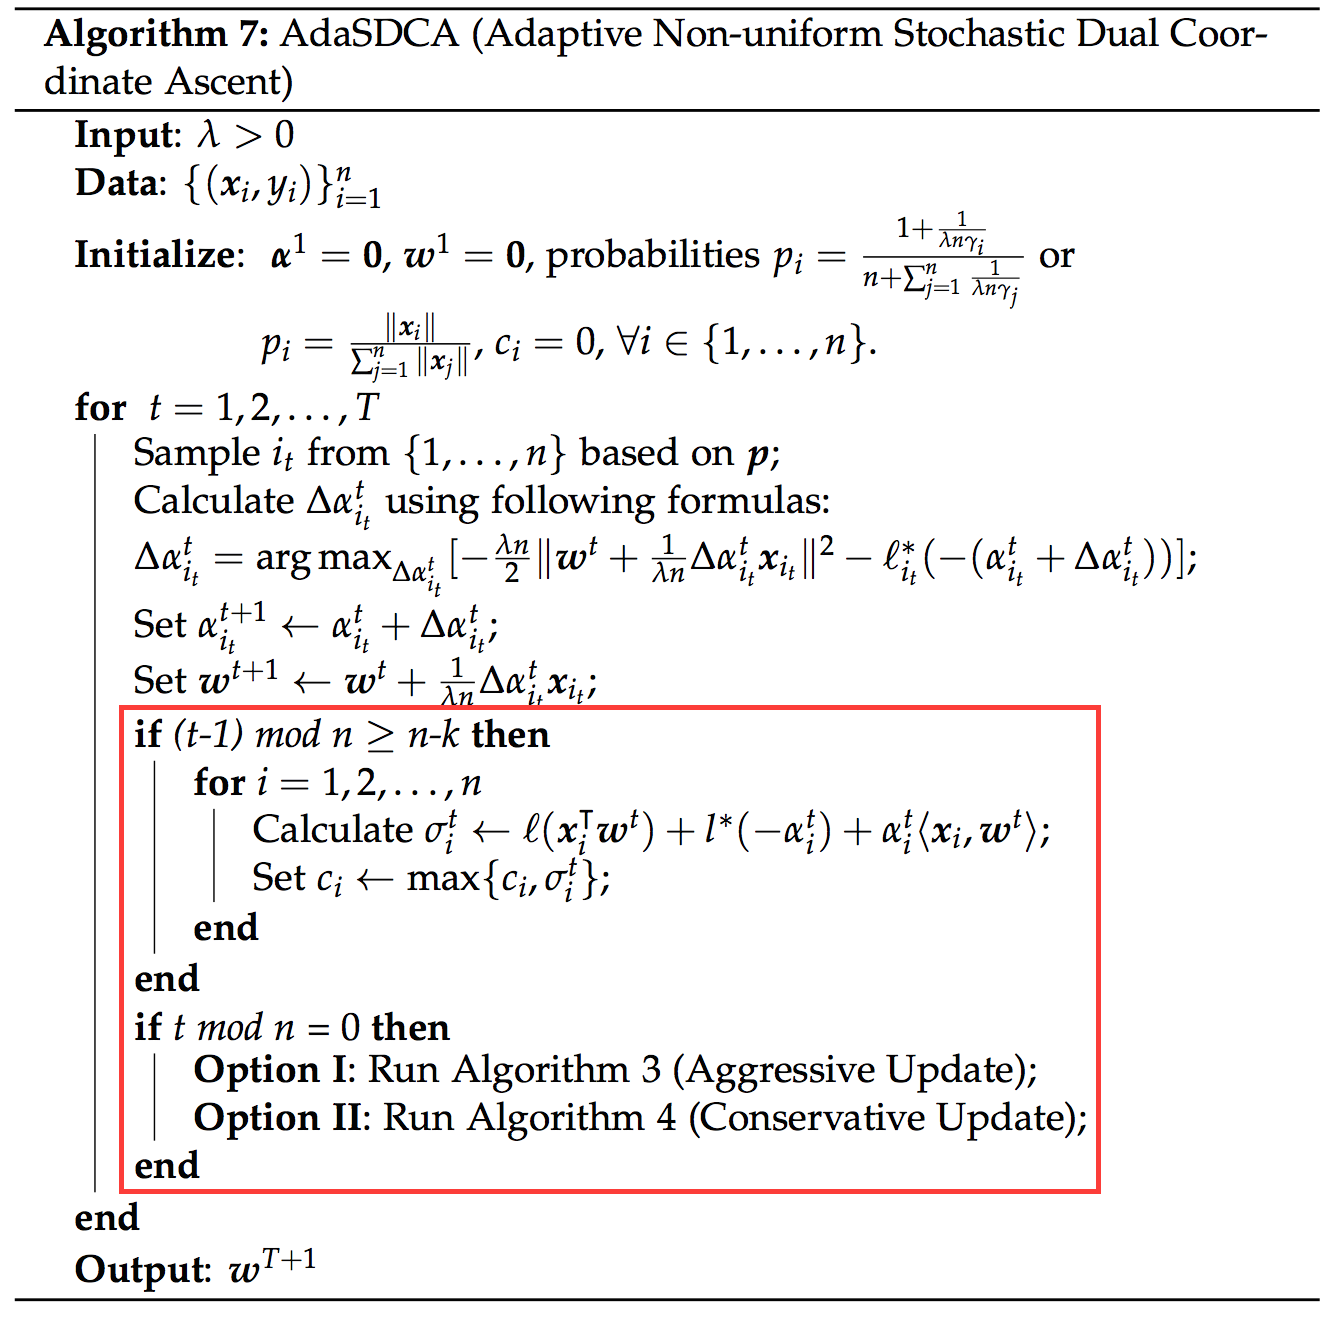
\includegraphics[height=0.8\textheight]{images/AdaSDCA.png} 
    \label{fig:AdaSDCA}
\end{figure}
\end{frame}

\begin{frame}{AdaSDCAS}
\begin{figure}[H]
        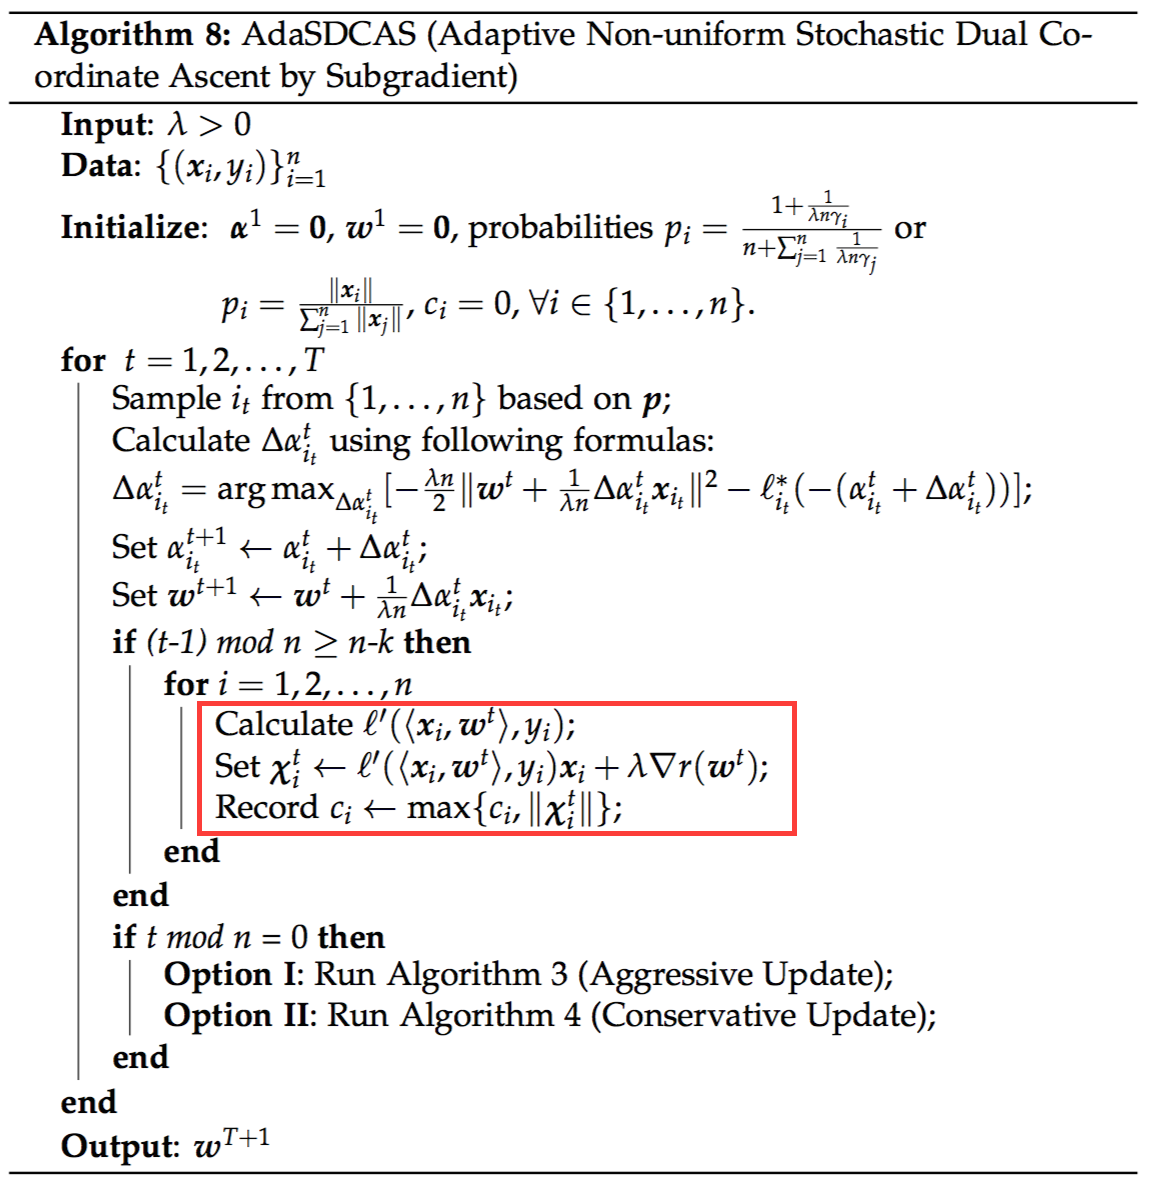
\includegraphics[height=0.8\textheight]{images/AdaSDCAS.png} 
    \label{fig:AdaSDCA}
\end{figure}
\end{frame}
